\documentclass[12pt]{article}
%\usepackage{fullpage}
\usepackage{epic}
\usepackage{eepic}
\usepackage{paralist}
\usepackage{graphicx}
\usepackage{algorithm,algorithmic}
\usepackage{tikz}
\usepackage{xcolor,colortbl}
\usepackage{wrapfig}
\usepackage{amsmath}

%%%%%%%%%%%%%%%%%%%%%%%%%%%%%%%%%%%%%%%%%%%%%%%%%%%%%%%%%%%%%%%%
% This is FULLPAGE.STY by H.Partl, Version 2 as of 15 Dec 1988.
% Document Style Option to fill the paper just like Plain TeX.

\typeout{Style Option FULLPAGE Version 2 as of 15 Dec 1988}

\topmargin 0pt
\advance \topmargin by -\headheight
\advance \topmargin by -\headsep

\textheight 8.9in

\oddsidemargin 0pt
\evensidemargin \oddsidemargin
\marginparwidth 0.5in

\textwidth 6.5in
%%%%%%%%%%%%%%%%%%%%%%%%%%%%%%%%%%%%%%%%%%%%%%%%%%%%%%%%%%%%%%%%

\pagestyle{empty}
\setlength{\oddsidemargin}{0in}
\setlength{\topmargin}{-0.8in}
\setlength{\textwidth}{6.8in}
\setlength{\textheight}{9.5in}


\def\ind{\hspace*{0.3in}}
\def\gap{0.1in}
\def\bigap{0.25in}
\newcommand{\Xomit}[1]{}


\begin{document}

\setlength{\parindent}{0in}
\addtolength{\parskip}{0.1cm}
\setlength{\fboxrule}{.5mm}\setlength{\fboxsep}{1.2mm}
\newlength{\boxlength}\setlength{\boxlength}{\textwidth}
\addtolength{\boxlength}{-4mm}
\begin{center}\framebox{\parbox{\boxlength}{{\bf
CS 4820, Spring 2018 \hfill Homework 3, Problem 2}\\
% TODO: fill in your own name, netID, and collaborators
Name: \\
NetID: \\
Collaborators:
}}
\end{center}
\vspace{5mm}

{\bf (3)} {\em (10 points)} \\
In the {\sc Tromino Tiling} problem one is given
a subset of a square grid, and one must decide 
whether the given subset can be tiled (i.e., 
covered without overlaps) by L-shaped trominoes.

The input to the problem can be given in the form 
of a $k \times n$ array of 0's and 1's. 
Denoting this array by $A$, the
entry $A[i,j]$ equals 1 if the grid cell in 
location $(i,j)$ belongs to the subset to be tiled, 
and if not then $A[i,j]=0$.

Design an algorithm to solve {\sc Tromino Tiling}
in time $O(n) \cdot 2^{O(k)}$.
Your algorithm only needs to output a simple ``yes''
or ``no'' answer indicating whether or not
the given subset of the grid can be tiled by 
L-shaped trominoes. In describing your algorithm, 
you may assume you have access to a subroutine
called {\sc WidthTwo} that solves the case when
$n$ (the width of the grid) is equal to 2, and 
$k$ (the grid's height) is an arbitrary positive
integer. The running time of the {\sc WidthTwo} 
subroutine is $O(k)$. You are \emph{not} responsible for
designing or analyzing the {\sc WidthTwo} 
subroutine; you are welcome to just assume it
exists and treat it as a ``black box.'' 

Note that the running time of the algorithm 
you are being asked to design is {\bf not 
polynomial in the input size}. It is linear
in $n$ but exponential in $k$. Partial credit
will be awarded for algorithms 
whose running time depends 
super-exponentially on $k$, or has
super-linear but still polynomial
dependence on $n$. No credit will be awarded
for algorithms whose running time is 
exponential in $n$. 

{\bf Example.} In the following example
$k=4$ and $n=6$, and the matrix $A$ is
given by
\[
  A = \begin{pmatrix}
    0 & 1 & 0 & 1 & 1 & 0 \\
    1 & 1 & 1 & 1 & 1 & 0 \\
    0 & 1 & 1 & 1 & 1 & 1 \\
    0 & 0 & 1 & 0 & 1 & 0 
  \end{pmatrix} .
\]
The region to be tiled
is the set of white squares in the left
figure below. The right figure illustrates
a tromino tiling of the region.

\vskip \gap

\begin{center}
\begin{minipage}{0.3\textwidth}
  \begin{tikzpicture}
    \draw[black] (0,0) grid (6,4);
    \filldraw[fill=black]
      (0,0) -- (2,0) -- (2,1) -- (1,1) -- (1,2) -- (0,2) -- cycle;
    \filldraw[fill=black]
      (3,0) rectangle (4,1);
    \filldraw[fill=black]
      (5,0) rectangle (6,1);
    \filldraw[fill=black]
      (0,3) rectangle (1,4);
    \filldraw[fill=black]
      (2,3) rectangle (3,4);
    \filldraw[fill=black]
      (5,2) rectangle (6,4);
  \end{tikzpicture}
\end{minipage}
\hspace*{0.1\textwidth}
\begin{minipage}{0.3\textwidth}
  \begin{tikzpicture}
    \filldraw[fill=black]
      (0,0) -- (2,0) -- (2,1) -- (1,1) -- (1,2) -- (0,2) -- cycle;
    \filldraw[fill=black]
      (3,0) rectangle (4,1);
    \filldraw[fill=black]
      (5,0) rectangle (6,1);
    \filldraw[fill=black]
      (0,3) rectangle (1,4);
    \filldraw[fill=black]
      (2,3) rectangle (3,4);
    \filldraw[fill=black]
      (5,2) rectangle (6,4);
    \filldraw[fill=yellow]
      (0,2) -- (2,2) -- (2,4) -- (1,4) -- (1,3) -- (0,3) -- cycle;
    \filldraw[fill=green!50]
      (2,2) -- (3,2) -- (3,1) -- (4,1) -- (4,3) -- (2,3) -- cycle;
    \filldraw[fill=pink]
      (1,1) -- (2,1) -- (2,0) -- (3,0) -- (3,2) -- (1,2) -- cycle;
    \filldraw[fill=blue!30]
      (3,3) -- (4,3) -- (4,2) -- (5,2) -- (5,4) -- (3,4) -- cycle;
    \filldraw[fill=brown!25]
      (4,0) -- (5,0) -- (5,1) -- (6,1) -- (6,2) -- (4,2) -- cycle;
    \draw[black] (0,0) grid (6,4);
  \end{tikzpicture}
\end{minipage}
\end{center}


\vskip \bigap

%% Your solution goes here.

\end{document}
